\chapter{Engenharia de Software e da Segurança}
\label{chap:engsoft}

\section{Análise dos Requisitos e Casos de Uso}
\label{sec:analreq}
De forma ao sistema corresponder a todas as expectativas, foi elaborada uma lista de requisitos composta por:

\begin{enumerate}
    \item Deve ser efetuadas comunicações(seguras) cliente-servidor e servidor-cliente.
    
    \item O utilizador deve realizar um registo inicial onde é gerado um par de chaves (pública e privada).
    
    \item O sistema deve permitir transações entre os seus clientes.
    
    \item O sistema deve lançar desafios de forma a criar novas moedas(fr€coin).
    
    \item O sistema deve suportar transações completamente anónimas entre utilizadores.
    
    \item A entidade central é também autoridade certificadora(servidor).
    
    \item O sistema deve ser implementado sobre curvas elípticas.
    
    \item O sistema deve suportar efetuar operações em simultâneo de forma a efetuar trabalho.
    
    \item O sistema deve lançar desafios sobre um tempo pré definido.
    
    \item O sistema deve ser capaz de controlar o número de fr€coin existente.
    
    \item O servidor deve ser uma entidade de confiança.
    
    \item O servidor deve conter informação acerca do nome do utilizador, a sua chave publica !!!!MAIS!!!!.
    
    \item O servidor deve conter todos os documentos das transações assinados pelas entidades que as efetuam.
    
    \item O cliente deve conter o seu par de chaves (pública e privada) e a chave pública do servidor.
    
\end{enumerate}

Quanto aos casos de uso, estes podem ser da forma:
!!!!!!!!!!!!!!!!!!!VERIFICAR DIAGRAMAS E MUDAR, ESTA NO PC BOINO OS DIAGRAMAS!!!!!!!!!!!!!!!!!!!


\begin{figure}[H]
\centering
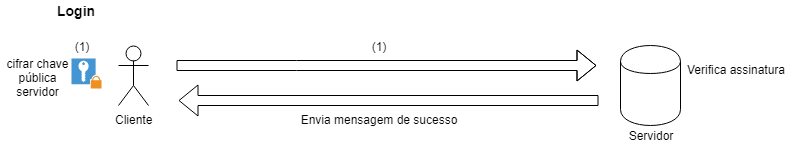
\includegraphics[width=.7\textwidth]{imagens/login.png}
\caption{Diagrama de login.}
\label{fig7}
\end{figure}


Sempre que se efetua o login, o utilizador envia um ficheiro cifrado com a sua chave privada, quando este pacote chega ao utilizador este verifica a assinatura e então é efetuado o login para esse cliente.

\begin{figure}[H]
\centering
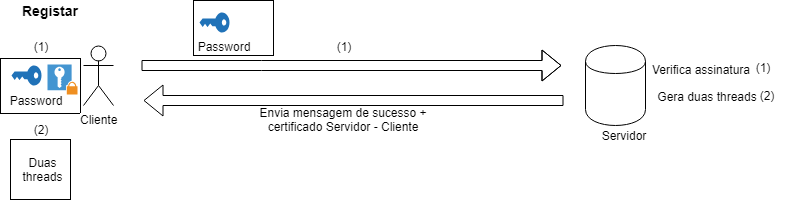
\includegraphics[width=.7\textwidth]{imagens/Registar.png}
\caption{Diagrama de Registar.}
\label{fig7}
\end{figure}


Neste diagrama, podemos verificar que o cliente irá efetuar uma comunicação com o servidor após este enviar uma mensagem encriptada. Ao chegar ao servidor é verificado e guardada o nome do utilizador e a sua chave pública correspondente, desta forma irá enviar uma resposta ao cliente e a partir desse momento podem assim efetuar uma ligação segura.

\begin{figure}[H]
\centering
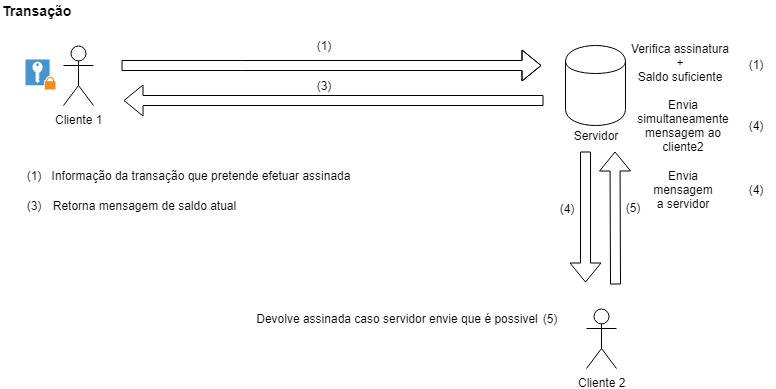
\includegraphics[width=.7\textwidth]{imagens/Transação.png}
\caption{Diagrama de transação.}
\label{fig7}
\end{figure}


Sempre que se pretende efetuar uma transação, o cliente envia uma mensagem ao servidor, assinada com a sua chave privada. Ao chegar ao servidor, este verifica a sua assinatura e se o cliente contem verba suficiente para esta transação. Se o cliente tiver esse montante descrito, é então enviada uma mensagem ao cliente 2(recetor) e é assinado por este. Caso não contenha a verba suficiente o cliente 2 apenas irá verificar a mensagem no entanto não a irá assinar. 
Todas as transações devem passar pelo servidor e com isso serem todas armazenadas no mesmo para mais tarde poderem ser verificadas.


\section{Outros Diagramas}
\label{sec:diagramas}


!!!!!!!!!!FAZER MODELOS DE ATAQUE??????ALGUNS BASICOS??????????!!!!!!!!!!

\section{Modelo do Sistema, Modelos de Ataque e propriedades de Segurança}
\label{sec:modelos}

\section{Modelação de Ataques}
\label{sec:ataques}

\section{Conclusão}
\label{sec:conclusao}

